% Options for packages loaded elsewhere
\PassOptionsToPackage{unicode}{hyperref}
\PassOptionsToPackage{hyphens}{url}
%
\documentclass[
  9pt,
  ignorenonframetext,
]{beamer}
\usepackage{pgfpages}
\setbeamertemplate{caption}[numbered]
\setbeamertemplate{caption label separator}{: }
\setbeamercolor{caption name}{fg=normal text.fg}
\beamertemplatenavigationsymbolsempty
% Prevent slide breaks in the middle of a paragraph
\widowpenalties 1 10000
\raggedbottom
\setbeamertemplate{note page}{\pagecolor{yellow!5}\Large\insertnote}\usepackage{palatino}
\setbeamertemplate{part page}{
  \centering
  \begin{beamercolorbox}[sep=16pt,center]{part title}
    \usebeamerfont{part title}\insertpart\par
  \end{beamercolorbox}
}
\setbeamertemplate{section page}{
  \centering
  \begin{beamercolorbox}[sep=12pt,center]{part title}
    \usebeamerfont{section title}\insertsection\par
  \end{beamercolorbox}
}
\setbeamertemplate{subsection page}{
  \centering
  \begin{beamercolorbox}[sep=8pt,center]{part title}
    \usebeamerfont{subsection title}\insertsubsection\par
  \end{beamercolorbox}
}
\AtBeginPart{
  \frame{\partpage}
}
\AtBeginSection{
  \ifbibliography
  \else
    \frame{\sectionpage}
  \fi
}
\AtBeginSubsection{
  \frame{\subsectionpage}
}
\usepackage{amsmath,amssymb}
\usepackage{lmodern}
\usepackage{iftex}
\ifPDFTeX
  \usepackage[T1]{fontenc}
  \usepackage[utf8]{inputenc}
  \usepackage{textcomp} % provide euro and other symbols
\else % if luatex or xetex
  \usepackage{unicode-math}
  \defaultfontfeatures{Scale=MatchLowercase}
  \defaultfontfeatures[\rmfamily]{Ligatures=TeX,Scale=1}
\fi
\usetheme[]{Copenhagen}
% Use upquote if available, for straight quotes in verbatim environments
\IfFileExists{upquote.sty}{\usepackage{upquote}}{}
\IfFileExists{microtype.sty}{% use microtype if available
  \usepackage[]{microtype}
  \UseMicrotypeSet[protrusion]{basicmath} % disable protrusion for tt fonts
}{}
\makeatletter
\@ifundefined{KOMAClassName}{% if non-KOMA class
  \IfFileExists{parskip.sty}{%
    \usepackage{parskip}
  }{% else
    \setlength{\parindent}{0pt}
    \setlength{\parskip}{6pt plus 2pt minus 1pt}}
}{% if KOMA class
  \KOMAoptions{parskip=half}}
\makeatother
\usepackage{xcolor}
\IfFileExists{xurl.sty}{\usepackage{xurl}}{} % add URL line breaks if available
\IfFileExists{bookmark.sty}{\usepackage{bookmark}}{\usepackage{hyperref}}
\hypersetup{
  pdfauthor={Joonas Laukka},
  hidelinks,
  pdfcreator={LaTeX via pandoc}}
\urlstyle{same} % disable monospaced font for URLs
\newif\ifbibliography
\usepackage{color}
\usepackage{fancyvrb}
\newcommand{\VerbBar}{|}
\newcommand{\VERB}{\Verb[commandchars=\\\{\}]}
\DefineVerbatimEnvironment{Highlighting}{Verbatim}{commandchars=\\\{\}}
% Add ',fontsize=\small' for more characters per line
\newenvironment{Shaded}{}{}
\newcommand{\AlertTok}[1]{\textcolor[rgb]{1.00,0.00,0.00}{\textbf{#1}}}
\newcommand{\AnnotationTok}[1]{\textcolor[rgb]{0.38,0.63,0.69}{\textbf{\textit{#1}}}}
\newcommand{\AttributeTok}[1]{\textcolor[rgb]{0.49,0.56,0.16}{#1}}
\newcommand{\BaseNTok}[1]{\textcolor[rgb]{0.25,0.63,0.44}{#1}}
\newcommand{\BuiltInTok}[1]{\textcolor[rgb]{0.00,0.50,0.00}{#1}}
\newcommand{\CharTok}[1]{\textcolor[rgb]{0.25,0.44,0.63}{#1}}
\newcommand{\CommentTok}[1]{\textcolor[rgb]{0.38,0.63,0.69}{\textit{#1}}}
\newcommand{\CommentVarTok}[1]{\textcolor[rgb]{0.38,0.63,0.69}{\textbf{\textit{#1}}}}
\newcommand{\ConstantTok}[1]{\textcolor[rgb]{0.53,0.00,0.00}{#1}}
\newcommand{\ControlFlowTok}[1]{\textcolor[rgb]{0.00,0.44,0.13}{\textbf{#1}}}
\newcommand{\DataTypeTok}[1]{\textcolor[rgb]{0.56,0.13,0.00}{#1}}
\newcommand{\DecValTok}[1]{\textcolor[rgb]{0.25,0.63,0.44}{#1}}
\newcommand{\DocumentationTok}[1]{\textcolor[rgb]{0.73,0.13,0.13}{\textit{#1}}}
\newcommand{\ErrorTok}[1]{\textcolor[rgb]{1.00,0.00,0.00}{\textbf{#1}}}
\newcommand{\ExtensionTok}[1]{#1}
\newcommand{\FloatTok}[1]{\textcolor[rgb]{0.25,0.63,0.44}{#1}}
\newcommand{\FunctionTok}[1]{\textcolor[rgb]{0.02,0.16,0.49}{#1}}
\newcommand{\ImportTok}[1]{\textcolor[rgb]{0.00,0.50,0.00}{\textbf{#1}}}
\newcommand{\InformationTok}[1]{\textcolor[rgb]{0.38,0.63,0.69}{\textbf{\textit{#1}}}}
\newcommand{\KeywordTok}[1]{\textcolor[rgb]{0.00,0.44,0.13}{\textbf{#1}}}
\newcommand{\NormalTok}[1]{#1}
\newcommand{\OperatorTok}[1]{\textcolor[rgb]{0.40,0.40,0.40}{#1}}
\newcommand{\OtherTok}[1]{\textcolor[rgb]{0.00,0.44,0.13}{#1}}
\newcommand{\PreprocessorTok}[1]{\textcolor[rgb]{0.74,0.48,0.00}{#1}}
\newcommand{\RegionMarkerTok}[1]{#1}
\newcommand{\SpecialCharTok}[1]{\textcolor[rgb]{0.25,0.44,0.63}{#1}}
\newcommand{\SpecialStringTok}[1]{\textcolor[rgb]{0.73,0.40,0.53}{#1}}
\newcommand{\StringTok}[1]{\textcolor[rgb]{0.25,0.44,0.63}{#1}}
\newcommand{\VariableTok}[1]{\textcolor[rgb]{0.10,0.09,0.49}{#1}}
\newcommand{\VerbatimStringTok}[1]{\textcolor[rgb]{0.25,0.44,0.63}{#1}}
\newcommand{\WarningTok}[1]{\textcolor[rgb]{0.38,0.63,0.69}{\textbf{\textit{#1}}}}
\usepackage{graphicx}
\makeatletter
\def\maxwidth{\ifdim\Gin@nat@width>\linewidth\linewidth\else\Gin@nat@width\fi}
\def\maxheight{\ifdim\Gin@nat@height>\textheight\textheight\else\Gin@nat@height\fi}
\makeatother
% Scale images if necessary, so that they will not overflow the page
% margins by default, and it is still possible to overwrite the defaults
% using explicit options in \includegraphics[width, height, ...]{}
\setkeys{Gin}{width=\maxwidth,height=\maxheight,keepaspectratio}
% Set default figure placement to htbp
\makeatletter
\def\fps@figure{htbp}
\makeatother
\setlength{\emergencystretch}{3em} % prevent overfull lines
\providecommand{\tightlist}{%
  \setlength{\itemsep}{0pt}\setlength{\parskip}{0pt}}
\setcounter{secnumdepth}{-\maxdimen} % remove section numbering
\ifLuaTeX
  \usepackage{selnolig}  % disable illegal ligatures
\fi

\title{Enforcing authorization checks with the type system}
\subtitle{Ghosts of Departed Proofs (GDP) about JWTs}
\author{Joonas Laukka}
\date{Jan 11, 2023}
\institute{Software Developer @ RELEX Solutions}

\begin{document}
\begin{frame}
%\frame{\titlepage}
\titlepage
\end{frame}

\begin{frame}{About this talk}
\protect\hypertarget{about-this-talk}{}
\begin{itemize}
\tightlist
\item
  Prerequisites:

  \begin{itemize}
  \tightlist
  \item
    Requires intermediate knowledge of Haskell
  \item
    Haskell 2010 and many of GHC Language Extensions
  \end{itemize}
\item
  Goals:

  \begin{itemize}
  \tightlist
  \item
    Sharing my excitement with GDP
  \item
    Solving an imaginary problem related to authorization with GDP
  \item
    Getting all of you interested in Ghosts of Departed Proofs
  \end{itemize}
\item
  Let's go on an adventure together!
\end{itemize}









\end{frame}

\begin{frame}{About this talk}
\protect\hypertarget{about-this-talk-1}{}

\includegraphics[width=\textwidth,height=0.8\textheight]{resources/meme-cropped.png}
\end{frame}

\begin{frame}{Contents}
\protect\hypertarget{contents}{}
\begin{enumerate}
\tightlist
\item
  Crash course to GDP
\item
  Domain specific knowledge: authorization and JWTs
\item
  Applying GDP to authorization
\end{enumerate}







\end{frame}

\begin{frame}{Crash course to GDP}
\protect\hypertarget{crash-course-to-gdp}{}
\begin{figure}
\centering
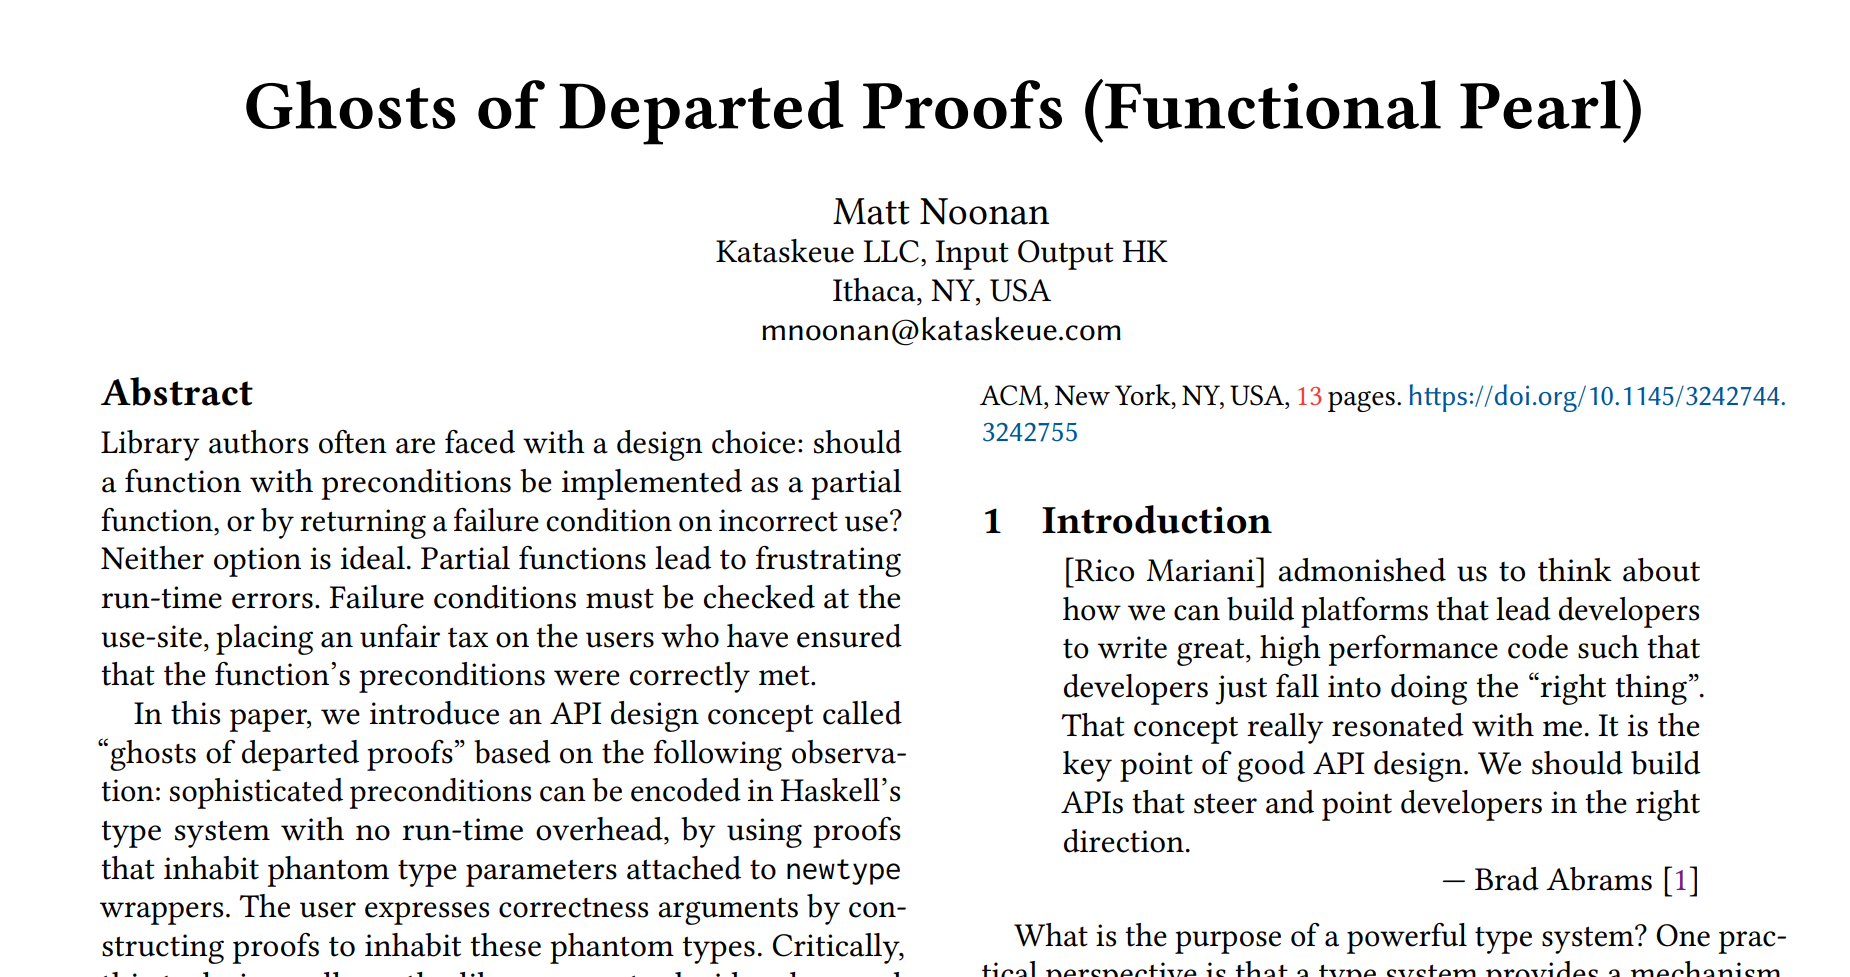
\includegraphics[width=\textwidth,height=0.8\textheight]{resources/gdp.png}
\caption{Published in 2018 by Matt Noonan}
\end{figure}






\end{frame}

\begin{frame}{Crash course to GDP}
\protect\hypertarget{crash-course-to-gdp-1}{}
\begin{figure}
\centering
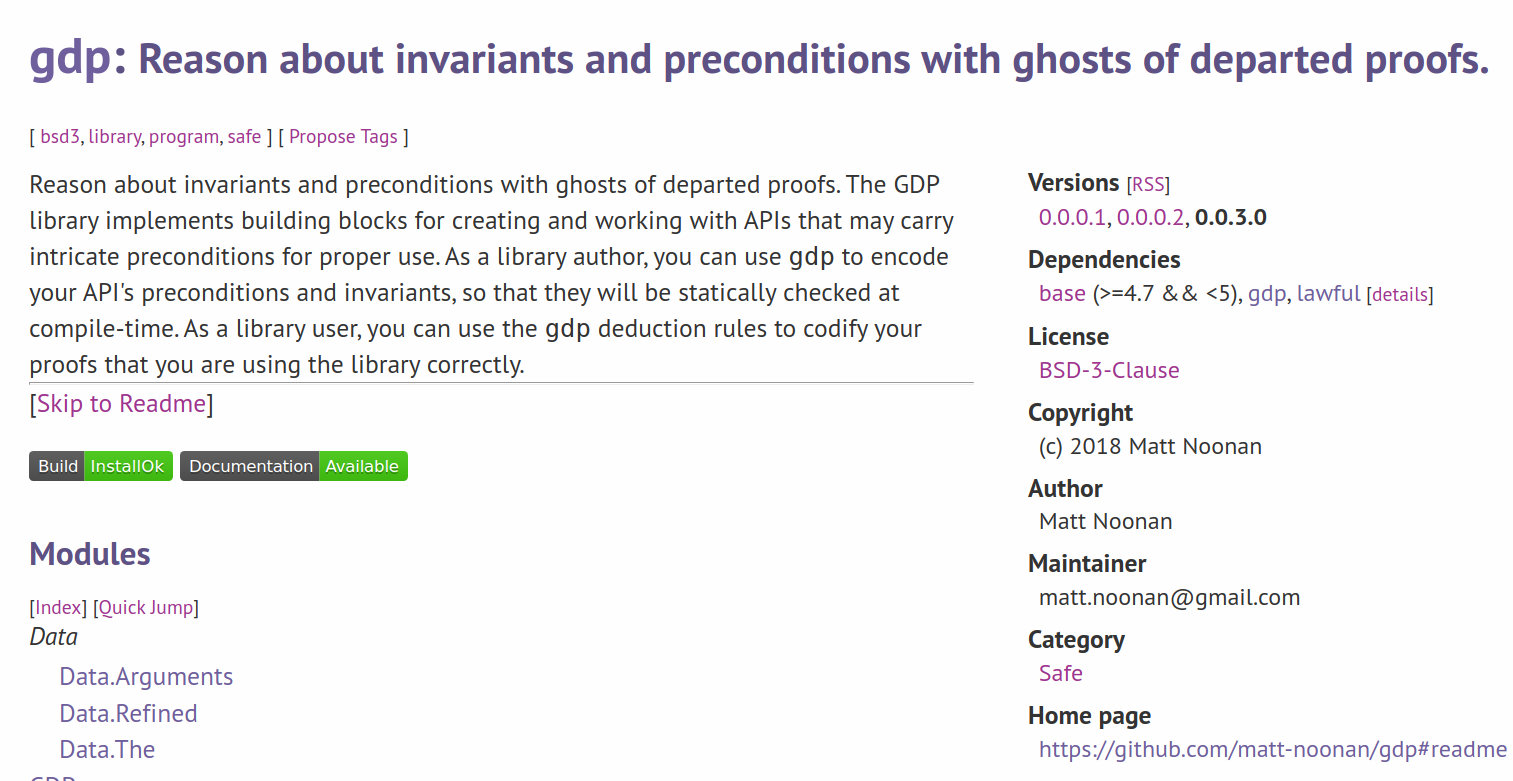
\includegraphics[width=\textwidth,height=0.8\textheight]{resources/gdp-library.png}
\caption{An auxiliary library is available on Hackage}
\end{figure}



\end{frame}

\begin{frame}[fragile]{Crash course to GDP}
\protect\hypertarget{crash-course-to-gdp-2}{}
\begin{quote}
What is the purpose of a powerful type system? One practical perspective
is that a type system provides a mechanism for enforcing program
invariants at compile time.
\end{quote}

Examples:

\begin{itemize}
\tightlist
\item
  Total functions with a limited domain

  \begin{itemize}
  \tightlist
  \item
    \texttt{headSafe\ ::\ NonEmpty\ a\ -\textgreater{}\ a}
  \end{itemize}
\item
  Functions that force the caller to handle a failure condition

  \begin{itemize}
  \tightlist
  \item
    \texttt{parse\ ::\ String\ -\textgreater{}\ Either\ Error\ a}
  \end{itemize}
\item
  Pure functions that have local, mutable state

  \begin{itemize}
  \tightlist
  \item
    \texttt{ST} monad
  \end{itemize}
\item
  Functions that require proof of authorization

  \begin{itemize}
  \tightlist
  \item
    \texttt{fireMissiles\ ::\ Proof\ AllowedToFire\ -\textgreater{}\ IO\ ()}
  \end{itemize}
\end{itemize}











\end{frame}

\begin{frame}{Crash course to GDP}
\protect\hypertarget{crash-course-to-gdp-3}{}
\begin{itemize}
\tightlist
\item
  Simple, everyday Haskell features already allow encoding very
  sophisticated invariants

  \begin{itemize}
  \tightlist
  \item
    These classic methods (such as newtype wrappers) are often
    sufficient
  \end{itemize}
\item
  But we're gonna play with GDP for the fun of it!

  \begin{itemize}
  \tightlist
  \item
    In the real world, the complexity of GDP itself might not be worth
    the value it brings (in most cases)
  \end{itemize}
\end{itemize}








\end{frame}

\begin{frame}{Crash course to GDP}
\protect\hypertarget{crash-course-to-gdp-4}{}

\begin{itemize}
\tightlist
\item
  GDP library attempts to make it easy to design APIs that are

  \begin{itemize}
  \tightlist
  \item
    \emph{safe}: we prevent the user from causing a run-time error
  \item
    \emph{ergonomic}: correct use of the API must not place an undue
    burden on the user
  \end{itemize}
\end{itemize}

Fundamental features of GDP API design concept:

\begin{itemize}
\tightlist
\item
  Naming objects
\item
  Properties and proofs are represented in code
\item
  Proofs are carried by phantom type parameters
\item
  Library-controlled APIs to create proofs
\item
  Combinators for manipulating ghost proofs
\end{itemize}












\end{frame}

\begin{frame}[fragile]{Crash course to GDP: naming objects}
\protect\hypertarget{crash-course-to-gdp-naming-objects}{}
\begin{Shaded}
\begin{Highlighting}[]
\KeywordTok{module} \DataTypeTok{Theory.Named}\NormalTok{ (}\DataTypeTok{Named}\NormalTok{, type (~~)}\NormalTok{, name) }\KeywordTok{where}

\KeywordTok{newtype} \DataTypeTok{Named}\NormalTok{ name a }\OtherTok{=} \DataTypeTok{Named}\NormalTok{ a}
\KeywordTok{type}\NormalTok{ role }\DataTypeTok{Named}\NormalTok{ nominal nominal}

\CommentTok{{-}{-} | An infix alias for \textquotesingle{}Named\textquotesingle{}.}
\KeywordTok{type}\NormalTok{ a }\OperatorTok{\textasciitilde{}\textasciitilde{}}\NormalTok{ name }\OtherTok{=} \DataTypeTok{Named}\NormalTok{ name a}

\CommentTok{{-}{-} | Compiler conjures a unique, existential name for }
\CommentTok{{-}{-} the value \textquotesingle{}x\textquotesingle{}.}
\CommentTok{{-}{-} }
\CommentTok{{-}{-} Similar to the well known ST trick.}
\OtherTok{name ::}\NormalTok{ a }\OtherTok{{-}\textgreater{}}\NormalTok{ (}\KeywordTok{forall}\NormalTok{ name}\OperatorTok{.}\NormalTok{ a }\OperatorTok{\textasciitilde{}\textasciitilde{}}\NormalTok{ name }\OtherTok{{-}\textgreater{}}\NormalTok{ t) }\OtherTok{{-}\textgreater{}}\NormalTok{ t}
\NormalTok{name x cont }\OtherTok{=}\NormalTok{ cont (coerce x)}
\end{Highlighting}
\end{Shaded}














\end{frame}

\begin{frame}{Crash course to GDP: naming objects}
\protect\hypertarget{crash-course-to-gdp-naming-objects-2}{}
\begin{quote}
In practice, it is as if the library has a secret supply of names, and
selects one to use in a manner that is not predictable to the user.
\end{quote}
\end{frame}

\begin{frame}[fragile]{Crash course to GDP: naming objects}
\protect\hypertarget{crash-course-to-gdp-naming-objects-3}{}
Naming allows attaching values to proofs about those values

\begin{Shaded}
\begin{Highlighting}[]
\NormalTok{isPrime }
\OtherTok{  ::}\NormalTok{ (}\DataTypeTok{Int} \OperatorTok{\textasciitilde{}\textasciitilde{}}\NormalTok{ n) }
  \OtherTok{{-}\textgreater{}} \DataTypeTok{Maybe}\NormalTok{ (}\DataTypeTok{Proof}\NormalTok{ (}\DataTypeTok{IsPrime}\NormalTok{ n))}

\NormalTok{isIssuedBy }
\OtherTok{  ::}\NormalTok{ (}\DataTypeTok{JWT} \OperatorTok{\textasciitilde{}\textasciitilde{}}\NormalTok{ token) }
  \OtherTok{{-}\textgreater{}} \DataTypeTok{Maybe}\NormalTok{ (}\DataTypeTok{Proof}\NormalTok{ (token }\OtherTok{\textasciigrave{}IsIssuedBy\textasciigrave{}}\NormalTok{ issuer))}
\end{Highlighting}
\end{Shaded}

The named object can be almost anything, e.g.~a function.


\end{frame}

\begin{frame}[fragile]{Crash course to GDP: naming objects}
\protect\hypertarget{crash-course-to-gdp-naming-objects-4}{}
\begin{Shaded}
\begin{Highlighting}[]
\NormalTok{usePrime }
\OtherTok{  ::}\NormalTok{ (}\DataTypeTok{Int} \OperatorTok{\textasciitilde{}\textasciitilde{}}\NormalTok{ n)}
  \OtherTok{{-}\textgreater{}} \DataTypeTok{Proof}\NormalTok{ (}\DataTypeTok{IsPrime}\NormalTok{ n)}
  \OtherTok{{-}\textgreater{}}\NormalTok{ m ()}

\NormalTok{example x }\OtherTok{=} 
\NormalTok{  name x }\OperatorTok{$}\NormalTok{ \textbackslash{}namedX }\OtherTok{{-}\textgreater{}}\NormalTok{ name }\DecValTok{2} \OperatorTok{$}\NormalTok{ \textbackslash{}namedTwo }\OtherTok{{-}\textgreater{}}
    \KeywordTok{let}\NormalTok{ twoIsPrime }\OtherTok{=}\NormalTok{ fromJust }\OperatorTok{$}\NormalTok{ isPrime namedTwo}
    \KeywordTok{in}\NormalTok{ usePrime namedX twoIsPrime}
\end{Highlighting}
\end{Shaded}

results in compiler error

\begin{verbatim}
• Couldn't match type ‘name1’ with ‘name’
      Expected: Int ~~ name1
        Actual: Int ~~ name
• In the first argument of ‘usePrime’, namely ‘namedX’
\end{verbatim}



\end{frame}

\begin{frame}[fragile]{Crash course to GDP: naming objects}
\protect\hypertarget{crash-course-to-gdp-naming-objects-5}{}
Results of library functions can also be named.

\begin{Shaded}
\begin{Highlighting}[]
\KeywordTok{newtype} \DataTypeTok{Inc}\NormalTok{ n }\OtherTok{=} \DataTypeTok{Inc} \DataTypeTok{Defn}

\OtherTok{increment ::}\NormalTok{ (}\DataTypeTok{Int} \OperatorTok{\textasciitilde{}\textasciitilde{}}\NormalTok{ n) }\OtherTok{{-}\textgreater{}}\NormalTok{ (}\DataTypeTok{Int} \OperatorTok{\textasciitilde{}\textasciitilde{}} \DataTypeTok{Inc}\NormalTok{ n)}
\NormalTok{increment n }\OtherTok{=}\NormalTok{ defn (the n }\OperatorTok{+} \DecValTok{1}\NormalTok{)}
\end{Highlighting}
\end{Shaded}









\end{frame}

\begin{frame}[fragile]{Crash course to GDP: unnaming objects}
\protect\hypertarget{crash-course-to-gdp-unnaming-objects}{}
\begin{Shaded}
\begin{Highlighting}[]
\KeywordTok{newtype} \DataTypeTok{Named}\NormalTok{ name a }\OtherTok{=} \DataTypeTok{Named}\NormalTok{ a}

\KeywordTok{class} \DataTypeTok{The}\NormalTok{ d a }\OperatorTok{|}\NormalTok{ d }\OtherTok{{-}\textgreater{}}\NormalTok{ a }\KeywordTok{where}
\OtherTok{  the ::}\NormalTok{ d }\OtherTok{{-}\textgreater{}}\NormalTok{ a}
\NormalTok{  default}\OtherTok{ the ::} \DataTypeTok{Coercible}\NormalTok{ d a }\OtherTok{=\textgreater{}}\NormalTok{ d }\OtherTok{{-}\textgreater{}}\NormalTok{ a}
\NormalTok{  the }\OtherTok{=}\NormalTok{ coerce}

\KeywordTok{instance} \DataTypeTok{The}\NormalTok{ (}\DataTypeTok{Named}\NormalTok{ name a) a}

\CommentTok{{-}{-} the :: (Int \textasciitilde{}\textasciitilde{} n) {-}\textgreater{} Int}
\CommentTok{{-}{-} the = coerce}
\end{Highlighting}
\end{Shaded}

This is useful when writing proof constructors.




\end{frame}

\begin{frame}[fragile]{Crash course to GDP: proofs}
\protect\hypertarget{crash-course-to-gdp-proofs}{}
\begin{Shaded}
\begin{Highlighting}[]
\KeywordTok{module} \DataTypeTok{Logic.Proof}\NormalTok{ (}\DataTypeTok{Proof}\NormalTok{, axiom) }\KeywordTok{where}

\CommentTok{{-}{-} | Value of type \textquotesingle{}Proof p\textquotesingle{} represents proof of @p@}
\KeywordTok{data} \DataTypeTok{Proof}\NormalTok{ p }\OtherTok{=} \DataTypeTok{QED}

\OtherTok{axiom ::} \DataTypeTok{Proof}\NormalTok{ p }
\NormalTok{axiom }\OtherTok{=} \DataTypeTok{QED}

\KeywordTok{module} \DataTypeTok{IsOdd}\NormalTok{ (}\DataTypeTok{IsOdd}\NormalTok{, isOdd)}

\CommentTok{{-}{-} | Proposition: integer is odd}
\KeywordTok{data} \DataTypeTok{IsOdd}\NormalTok{ n}

\OtherTok{isOdd ::}\NormalTok{ (}\DataTypeTok{Int} \OperatorTok{\textasciitilde{}\textasciitilde{}}\NormalTok{ n) }\OtherTok{{-}\textgreater{}} \DataTypeTok{Maybe}\NormalTok{ (}\DataTypeTok{Proof}\NormalTok{ (}\DataTypeTok{IsOdd}\NormalTok{ n))}
\NormalTok{isOdd n }\OtherTok{=} \KeywordTok{if} \FunctionTok{odd}\NormalTok{ (the n) }
  \KeywordTok{then} \DataTypeTok{Just}\NormalTok{ axiom}
  \KeywordTok{else} \DataTypeTok{Nothing}
\end{Highlighting}
\end{Shaded}





\end{frame}

\begin{frame}[fragile]{Crash course to GDP: proofs}
\protect\hypertarget{crash-course-to-gdp-proofs-1}{}
Values can be attached with proofs via \texttt{:::}.

\begin{Shaded}
\begin{Highlighting}[]
\KeywordTok{newtype}\NormalTok{ a }\OperatorTok{:::}\NormalTok{ p }\OtherTok{=} \DataTypeTok{SuchThat}\NormalTok{ a}

\NormalTok{usePrime }
\OtherTok{  ::}\NormalTok{ (}\DataTypeTok{Int} \OperatorTok{\textasciitilde{}\textasciitilde{}}\NormalTok{ n)}
  \OtherTok{{-}\textgreater{}} \DataTypeTok{Proof}\NormalTok{ (}\DataTypeTok{IsPrime}\NormalTok{ n)}
  \OtherTok{{-}\textgreater{}}\NormalTok{ m ()}

\NormalTok{usePrime}
\OtherTok{  ::}\NormalTok{ (}\DataTypeTok{Int} \OperatorTok{\textasciitilde{}\textasciitilde{}}\NormalTok{ n }\OperatorTok{:::} \DataTypeTok{IsPrime}\NormalTok{ n)}
  \OtherTok{{-}\textgreater{}}\NormalTok{ m ()}

\OtherTok{(...)  ::}\NormalTok{ a }\OtherTok{{-}\textgreater{}} \DataTypeTok{Proof}\NormalTok{ p }\OtherTok{{-}\textgreater{}}\NormalTok{ (a }\OperatorTok{:::}\NormalTok{ p)}

\OtherTok{exorcise ::}\NormalTok{ (a }\OperatorTok{:::}\NormalTok{ p) }\OtherTok{{-}\textgreater{}}\NormalTok{ a}
\OtherTok{conjure  ::}\NormalTok{ (a }\OperatorTok{:::}\NormalTok{ p) }\OtherTok{{-}\textgreater{}} \DataTypeTok{Proof}\NormalTok{ p}
\end{Highlighting}
\end{Shaded}








\end{frame}

\begin{frame}[fragile]{Crash course to GDP: proofs}
\protect\hypertarget{crash-course-to-gdp-proofs-2}{}

The proof attached to a value can be completely unrelated to it but
usually there exists a clear connection:

\begin{Shaded}
\begin{Highlighting}[]
\CommentTok{{-}{-} "A value of type Int, named n, such that n is a prime"}
\NormalTok{(}\DataTypeTok{Int} \OperatorTok{\textasciitilde{}\textasciitilde{}}\OtherTok{ n :::} \DataTypeTok{IsPrime}\NormalTok{ n)}

\CommentTok{{-}{-} "A value of type Int, named n, such that the increment of n is odd"}
\NormalTok{(}\DataTypeTok{Int} \OperatorTok{\textasciitilde{}\textasciitilde{}}\OtherTok{ n :::} \DataTypeTok{IsOdd}\NormalTok{ (}\DataTypeTok{Inc}\NormalTok{ n))}

\CommentTok{{-}{-} "A value of type Int, named n, such that the sun is shining"}
\NormalTok{(}\DataTypeTok{Int} \OperatorTok{\textasciitilde{}\textasciitilde{}}\OtherTok{ n :::} \DataTypeTok{SunIsShining}\NormalTok{)}
\end{Highlighting}
\end{Shaded}




\end{frame}

\begin{frame}[fragile]{Crash course to GDP: proofs}
\protect\hypertarget{crash-course-to-gdp-proofs-3}{}
\begin{Shaded}
\begin{Highlighting}[]
\KeywordTok{module} \DataTypeTok{Logic.Propositional} \KeywordTok{where}

\CommentTok{{-}{-} Logical connectives}
\KeywordTok{data}\NormalTok{ p }\OperatorTok{\&\&}\NormalTok{ q }
\KeywordTok{data}\NormalTok{ p }\OperatorTok{||}\NormalTok{ q }
\KeywordTok{data}\NormalTok{ p }\OperatorTok{{-}{-}\textgreater{}}\NormalTok{ q}
\KeywordTok{data}\NormalTok{ p }\OperatorTok{==}\NormalTok{ q}

\CommentTok{{-}{-} Introduce premises}
\NormalTok{introImpl}
\OtherTok{  ::}\NormalTok{ (}\DataTypeTok{Proof}\NormalTok{ p }\OtherTok{{-}\textgreater{}} \DataTypeTok{Proof}\NormalTok{ q)}
  \OtherTok{{-}\textgreater{}} \DataTypeTok{Proof}\NormalTok{ (p }\OperatorTok{{-}{-}\textgreater{}}\NormalTok{ q)}
\CommentTok{{-}{-} Deduction rules}
\NormalTok{elimImpl}
\OtherTok{  ::} \DataTypeTok{Proof}\NormalTok{ p}
  \OtherTok{{-}\textgreater{}} \DataTypeTok{Proof}\NormalTok{ (p }\OperatorTok{{-}{-}\textgreater{}}\NormalTok{ q)}
  \OtherTok{{-}\textgreater{}} \DataTypeTok{Proof}\NormalTok{ q}
\end{Highlighting}
\end{Shaded}





\end{frame}

\begin{frame}[fragile]{Crash course to GDP: proofs}
\protect\hypertarget{crash-course-to-gdp-proofs-4}{}
The functions in \texttt{Logic.Propositional} allow building proofs from
other proofs:

\begin{Shaded}
\begin{Highlighting}[]
\KeywordTok{data} \DataTypeTok{IsNatural}\NormalTok{ n}

\CommentTok{{-}{-} Increment of a natural number is a natural number.}
\OtherTok{naturalInc ::} \DataTypeTok{Proof}\NormalTok{ (}\DataTypeTok{IsNatural}\NormalTok{ n }\OperatorTok{{-}{-}\textgreater{}} \DataTypeTok{IsNatural}\NormalTok{ (}\DataTypeTok{Inc}\NormalTok{ n))}
\NormalTok{naturalInc }\OtherTok{=}\NormalTok{ axiom}

\NormalTok{incrementNatural}
\OtherTok{  ::}\NormalTok{ (}\DataTypeTok{Int} \OperatorTok{\textasciitilde{}\textasciitilde{}}\NormalTok{ n }\OperatorTok{:::} \DataTypeTok{IsNatural}\NormalTok{ n) }
  \OtherTok{{-}\textgreater{}}\NormalTok{ (}\DataTypeTok{Int} \OperatorTok{\textasciitilde{}\textasciitilde{}} \DataTypeTok{Inc}\NormalTok{ n }\OperatorTok{:::} \DataTypeTok{IsNatural}\NormalTok{ (}\DataTypeTok{Inc}\NormalTok{ n))}
\NormalTok{incrementNatural number }\OtherTok{=}
  \KeywordTok{let}\NormalTok{ proof       }\OtherTok{=}\NormalTok{ conjure number}
\NormalTok{      incremented }\OtherTok{=}\NormalTok{ increment }\OperatorTok{$}\NormalTok{ exorcise number}
  \KeywordTok{in}\NormalTok{ incremented }\OperatorTok{...\textgreater{}}\NormalTok{ (}\OtherTok{\textasciigrave{}elimImpl\textasciigrave{}}\NormalTok{ naturalInc)}
\end{Highlighting}
\end{Shaded}




\end{frame}

\begin{frame}[fragile]{Crash course to GDP: proofs}
\protect\hypertarget{crash-course-to-gdp-proofs-5}{}
\begin{block}{Writing axioms in Haskell}
\protect\hypertarget{writing-axioms-in-haskell}{}
\hfill\break

\begin{quote}
\textbf{Increment of a natural number is a natural number.}
\end{quote}

\[ n \in \mathbb{N} \implies n + 1 \in \mathbb{N} \]\\

\begin{Shaded}
\begin{Highlighting}[]
\NormalTok{naturalInc }
\OtherTok{  ::} \DataTypeTok{Proof}\NormalTok{ (}\DataTypeTok{IsNatural}\NormalTok{ n }\OperatorTok{{-}{-}\textgreater{}} \DataTypeTok{IsNatural}\NormalTok{ (}\DataTypeTok{Inc}\NormalTok{ n))}
\NormalTok{naturalInc }\OtherTok{=}\NormalTok{ axiom}
\end{Highlighting}
\end{Shaded}
\end{block}


\end{frame}

\begin{frame}[fragile]{Crash course to GDP: proofs}
\protect\hypertarget{crash-course-to-gdp-proofs-6}{}
\begin{block}{Writing axioms in Haskell}
\protect\hypertarget{writing-axioms-in-haskell-1}{}
\hfill\break

\begin{quote}
\textbf{User can delete applications if his token was issued by Azure or
OKTA}\\
\strut \\
\end{quote}

\begin{Shaded}
\begin{Highlighting}[]
\KeywordTok{data} \DataTypeTok{CanDeleteApps}\NormalTok{ token}

\NormalTok{canDeleteApps }
\OtherTok{  ::} \DataTypeTok{Proof}\NormalTok{ (}
\NormalTok{       ( token }\OtherTok{\textasciigrave{}IssuedBy\textasciigrave{}} \StringTok{"azure"} 
         \OperatorTok{||}\NormalTok{ token }\OtherTok{\textasciigrave{}IssuedBy\textasciigrave{}} \StringTok{"okta"}
\NormalTok{       )}
       \OperatorTok{{-}{-}\textgreater{}}
\NormalTok{       (}\DataTypeTok{CanDeleteApps}\NormalTok{ token)}
\NormalTok{     )}
\NormalTok{canDeleteApps }\OtherTok{=}\NormalTok{ axiom}
\end{Highlighting}
\end{Shaded}
\end{block}



\end{frame}

\begin{frame}{Domain specific knowledge: What is authorization?}
\protect\hypertarget{domain-specific-knowledge-what-is-authorization}{}
According to wikipedia:\\
\strut \\

\begin{quote}
``Authorization is the function of specifying access rights/privileges
to resources.''
\end{quote}

In practice,\\
\strut \\

\begin{quote}
``During operation, the system uses the access control rules to decide
whether access requests from authenticated consumers shall be approved
(granted) or disapproved (rejected).''
\end{quote}



\end{frame}

\begin{frame}{Domain specific knowledge: JSON Web Tokens}
\protect\hypertarget{domain-specific-knowledge-json-web-tokens}{}
\begin{figure}
\centering

\includegraphics[width=0.2\textwidth,height=\textheight]{resources/oauth.png}
\caption{OAuth is an industry standard protocol for authorization}
\end{figure}

\begin{quote}
``JSON Web Tokens (JWTs) are an open, industry standard RFC 7519 method
for representing claims securely between two parties.''
\end{quote}

\begin{itemize}
\tightlist
\item
  JSON Web Tokens are everywhere!

  \begin{itemize}
  \tightlist
  \item
    OAuth 2.0 access tokens are often JWTs
  \item
    OpenID Connect identity tokens are always JWTs
  \end{itemize}
\item
  JWT claims can carry information needed for authorization decisions
\item
  I chose to focus on JWTs in this talk!
\end{itemize}






\end{frame}

\begin{frame}{Domain specific knowledge: JWT structure}
\protect\hypertarget{domain-specific-knowledge-jwt-structure}{}
\begin{figure}
\centering
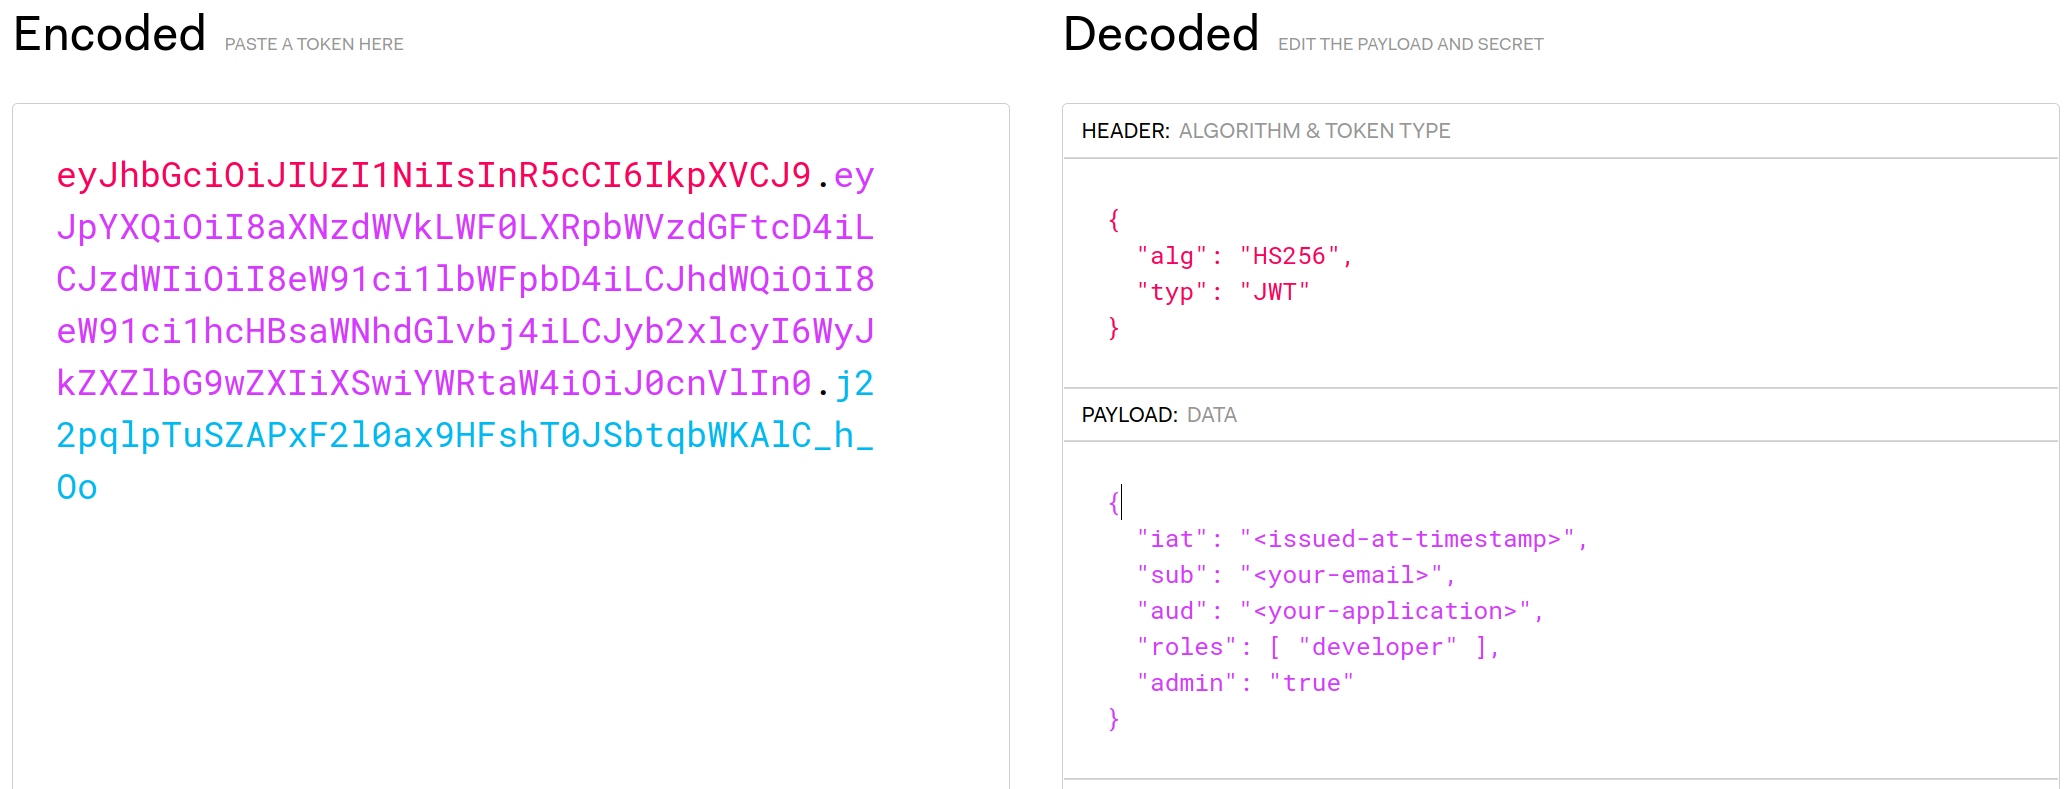
\includegraphics[width=\textwidth,height=1.2\textheight]{resources/jwt-single-picture.png}
\caption{An example JWT}
\end{figure}







\end{frame}

\begin{frame}[fragile]{Domain specific knowledge: JWTs in Haskell
ecosystem}
\protect\hypertarget{domain-specific-knowledge-jwts-in-haskell-ecosystem}{}
\begin{itemize}
\tightlist
\item
  A hackage package called \emph{jose} provides excellent primitive
  functions for

  \begin{itemize}
  \tightlist
  \item
    validating/verifying tokens
  \item
    extracting claims from valid tokens
  \end{itemize}
\end{itemize}

\begin{block}{jose types}
\protect\hypertarget{jose-types}{}
\begin{Shaded}
\begin{Highlighting}[]
\CommentTok{{-}{-} | RFC 7517 §4.  JSON Web Key (JWK) Format}
\KeywordTok{data} \DataTypeTok{JWK} 

\CommentTok{{-}{-} | A digitally signed or MACed JWT}
\KeywordTok{type} \DataTypeTok{SignedJWT} \OtherTok{=} \DataTypeTok{CompactJWS} \DataTypeTok{JWSHeader}

\CommentTok{{-}{-} | The JWT Claims Set represents a JSON object }
\KeywordTok{data} \DataTypeTok{ClaimsSet}
\end{Highlighting}
\end{Shaded}
\end{block}






\end{frame}

\begin{frame}[fragile]{Problem statement}
\protect\hypertarget{problem-statement}{}
Let's say we are developing a Haskell application that accepts JWTs from
two distinct Authorization Servers, \texttt{Azure\ AD} and
\texttt{OKTA}.

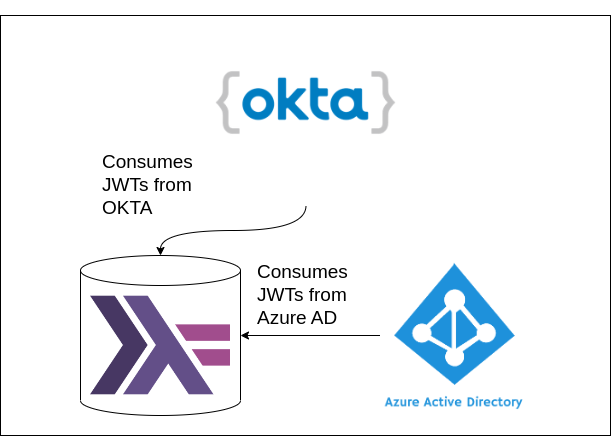
\includegraphics[width=\textwidth,height=0.7\textheight]{resources/problem-statement.drawio.png}





\end{frame}

\begin{frame}{Problem statement}
\protect\hypertarget{problem-statement-1}{}
\begin{itemize}
\tightlist
\item
  Let's assume that both Azure AD and OKTA maintain a record of which
  roles a user is assigned to
\item
  And those roles are sent as claims in the JWTs issued by them
\item
  Unfortunately, the schemas of the payloads don't quite match.
\end{itemize}



\end{frame}

\begin{frame}[fragile]{Problem statement: JWTs from Azure}
\protect\hypertarget{problem-statement-jwts-from-azure}{}
The payload of a JWT issued by Azure looks like this:

\begin{Shaded}
\begin{Highlighting}[]
\FunctionTok{\{}
  \DataTypeTok{"iss"}\FunctionTok{:} \StringTok{"Azure AD"}\FunctionTok{,}
  \DataTypeTok{"sub"}\FunctionTok{:} \StringTok{"\textless{}your{-}username\textgreater{}"}\FunctionTok{,}
  \DataTypeTok{"iat"}\FunctionTok{:} \StringTok{"\textless{}issued{-}at{-}timestamp\textgreater{}"}\FunctionTok{,}
  \DataTypeTok{"aud"}\FunctionTok{:} \StringTok{"\textless{}your{-}application\textgreater{}"}\FunctionTok{,}
  \DataTypeTok{"roles"}\FunctionTok{:} \OtherTok{[}
     \StringTok{"\textless{}role{-}name\textgreater{}"}\OtherTok{,}
     \StringTok{"\textless{}another{-}role{-}name\textgreater{}"}
  \OtherTok{]}
\FunctionTok{\}}
\end{Highlighting}
\end{Shaded}

\begin{itemize}
\tightlist
\item
  All of the roles that the user is assigned to are listed in the
  \texttt{roles} claim
\end{itemize}





\end{frame}

\begin{frame}[fragile]{Problem statement: JWTs from OKTA}
\protect\hypertarget{problem-statement-jwts-from-okta}{}
The payload of a JWT issued by OKTA looks like this:

\begin{Shaded}
\begin{Highlighting}[]
\FunctionTok{\{}
  \DataTypeTok{"iss"}\FunctionTok{:} \StringTok{"OKTA"}\FunctionTok{,}
  \DataTypeTok{"sub"}\FunctionTok{:} \StringTok{"\textless{}your{-}username\textgreater{}"}\FunctionTok{,}
  \DataTypeTok{"iat"}\FunctionTok{:} \StringTok{"\textless{}issued{-}at{-}timestamp\textgreater{}"}\FunctionTok{,}
  \DataTypeTok{"aud"}\FunctionTok{:} \StringTok{"\textless{}your{-}application\textgreater{}"}\FunctionTok{,}
  \DataTypeTok{"\textless{}role{-}name\textgreater{}"}\FunctionTok{:} \StringTok{"true"}\FunctionTok{,}
  \DataTypeTok{"\textless{}another{-}role{-}name\textgreater{}"}\FunctionTok{:} \StringTok{"false"}
\FunctionTok{\}}
\end{Highlighting}
\end{Shaded}

\begin{itemize}
\tightlist
\item
  Each role has its own claim in the JWT

  \begin{itemize}
  \tightlist
  \item
    The claim is named according to the name of the role
  \item
    The value of the claim is binary The user either (true or false)
  \end{itemize}
\end{itemize}






\end{frame}

\begin{frame}{Problem statement}
\protect\hypertarget{problem-statement-2}{}
\begin{block}{Problem}
\protect\hypertarget{problem}{}
Given that you receive a JWT from the user as input, how would you write
a function that can only be run if the user\\
\strut \\

\begin{itemize}
\tightlist
\item
  is an \textbf{administrator} according to Azure?
\item
  is an \textbf{administrator} or \textbf{developer} according to OKTA?
\item
  is an \textbf{administrator} according to either Azure or OKTA?
\end{itemize}
\end{block}





\end{frame}

\begin{frame}[fragile]{Applying GDP to authorization}
\protect\hypertarget{applying-gdp-to-authorization}{}
For a simple ad-hoc solution, we need

\begin{enumerate}
\tightlist
\item
  properties about JWTs such as

  \begin{itemize}
  \tightlist
  \item
    \texttt{data\ IssuedBy\ token\ source}
  \item
    \texttt{data\ HasAzureRole\ claims\ roleName}
  \item
    \texttt{data\ HasOktaRole\ claims\ roleName}
  \end{itemize}
\item
  names such as

  \begin{itemize}
  \tightlist
  \item
    \texttt{newtype\ ClaimsOf\ token\ =\ ClaimsOf\ Defn}
  \end{itemize}
\item
  properties about permissions such as

  \begin{itemize}
  \tightlist
  \item
    \texttt{data\ CanDeleteApps\ token}
  \end{itemize}
\end{enumerate}





\end{frame}

\begin{frame}[fragile]{Applying GDP to authorization: validation}
\protect\hypertarget{applying-gdp-to-authorization-validation}{}
\begin{Shaded}
\begin{Highlighting}[]
\KeywordTok{module} \DataTypeTok{Validation.IssuedBy} 
\NormalTok{  (}\DataTypeTok{IssuedBy}\NormalTok{, }\DataTypeTok{ClaimsOf}\NormalTok{, getClaimsOf) }\KeywordTok{where}

\KeywordTok{data} \DataTypeTok{IssuedBy}\NormalTok{ token (}\OtherTok{issuer ::} \DataTypeTok{Symbol}\NormalTok{)}

\KeywordTok{newtype} \DataTypeTok{ClaimsOf}\NormalTok{ token }\OtherTok{=} \DataTypeTok{ClaimsOf} \DataTypeTok{Defn}

\CommentTok{{-}{-} \textgreater{} getClaimsOf @"azure" token}
\CommentTok{{-}{-} }
\CommentTok{{-}{-} provides a proof if token was signed by Azure}
\NormalTok{getClaimsOf}
\OtherTok{  ::} \KeywordTok{forall}\NormalTok{ issuer token settings m}\OperatorTok{.}
\NormalTok{      ( }\DataTypeTok{KnownSymbol}\NormalTok{ issuer, }\DataTypeTok{MonadReader}\NormalTok{ s m}
\NormalTok{      , }\DataTypeTok{HasJWK}\NormalTok{ issuer s}
\NormalTok{      )}
  \OtherTok{=\textgreater{}}\NormalTok{ (}\DataTypeTok{SignedJWT} \OperatorTok{\textasciitilde{}\textasciitilde{}}\NormalTok{ token)}
  \OtherTok{{-}\textgreater{}}\NormalTok{ m (}\DataTypeTok{Maybe}\NormalTok{ (}
      \DataTypeTok{ClaimsSet} \OperatorTok{\textasciitilde{}\textasciitilde{}} \DataTypeTok{ClaimsOf}\NormalTok{ token }\OperatorTok{:::}\NormalTok{ (token }\OtherTok{\textasciigrave{}IssuedBy\textasciigrave{}}\NormalTok{ issuer))}
\NormalTok{     )}
\end{Highlighting}
\end{Shaded}







\end{frame}

\begin{frame}[fragile]{Applying GDP to authorization: Azure role}
\protect\hypertarget{applying-gdp-to-authorization-azure-role}{}
\begin{Shaded}
\begin{Highlighting}[]
\KeywordTok{module} \DataTypeTok{Validation.Azure.HasRole} 
\NormalTok{  (}\DataTypeTok{HasAzureRole}\NormalTok{, hasAzureRole) }\KeywordTok{where}

\KeywordTok{data} \DataTypeTok{HasAzureRole}\NormalTok{ claims (}\OtherTok{roleName ::} \DataTypeTok{Symbol}\NormalTok{)}

\CommentTok{{-}{-} @}
\CommentTok{{-}{-}   mAzureClaims \textless{}{-} getClaimsOf @"azure" token}
\CommentTok{{-}{-}   case mAzureClaims of }
\CommentTok{{-}{-}     Just claims {-}\textgreater{} hasAzureRole @"developer" claims}
\CommentTok{{-}{-} @}
\NormalTok{hasAzureRole}
\OtherTok{  ::} \KeywordTok{forall}\NormalTok{ roleName token}\OperatorTok{.} \DataTypeTok{KnownSymbol}\NormalTok{ roleName }
  \OtherTok{=\textgreater{}}\NormalTok{ (}\DataTypeTok{ClaimsSet} \OperatorTok{\textasciitilde{}\textasciitilde{}} \DataTypeTok{ClaimsOf}\NormalTok{ token }\OperatorTok{:::}\NormalTok{ (token }\OtherTok{\textasciigrave{}IssuedBy\textasciigrave{}} \StringTok{"azure"}\NormalTok{))}
  \CommentTok{{-}{-} \^{} Only accepts claims from a JWT issued by Azure}
  \OtherTok{{-}\textgreater{}} \DataTypeTok{Maybe}\NormalTok{ (}\DataTypeTok{Proof}\NormalTok{ (}\DataTypeTok{ClaimsOf}\NormalTok{ token }\OtherTok{\textasciigrave{}HasAzureRole\textasciigrave{}}\NormalTok{ roleName))}
\end{Highlighting}
\end{Shaded}






\end{frame}

\begin{frame}[fragile]{Applying GDP to authorization: Azure role}
\protect\hypertarget{applying-gdp-to-authorization-azure-role-1}{}
If we mix up claims from Azure and OKTA:

\begin{Shaded}
\begin{Highlighting}[]
\NormalTok{example jwt }\OtherTok{=} 
\NormalTok{  name jwt }\OperatorTok{$}\NormalTok{ \textbackslash{}namedJwt }\OtherTok{{-}\textgreater{}}
\NormalTok{    mOktaClaims }\OtherTok{\textless{}{-}}\NormalTok{ getClaimsOf }\OperatorTok{@}\StringTok{"okta"}\NormalTok{ namedJwt}
    \KeywordTok{case}\NormalTok{ mOktaClaims }\KeywordTok{of} 
      \DataTypeTok{Just}\NormalTok{ oktaClaims }\OtherTok{{-}\textgreater{}}\NormalTok{ hasAzureRole }\OperatorTok{@}\StringTok{"developer"}\NormalTok{ oktaClaims}
\end{Highlighting}
\end{Shaded}

the compiler screams at us

\begin{verbatim}
• Couldn't match type ‘"okta"’ with ‘"azure"’
  Expected: (ClaimsSet ~~ ClaimsOf name) ::: IssuedBy name "azure"
    Actual: (ClaimsSet ~~ ClaimsOf name) ::: IssuedBy name "okta"
• In the second argument of ‘hasAzureRole’, namely ‘oktaClaims’
  In the expression: hasAzureRole @"developer" oktaClaims
\end{verbatim}



\end{frame}

\begin{frame}[fragile]{Applying GDP to authorization: OKTA role}
\protect\hypertarget{applying-gdp-to-authorization-okta-role}{}
\begin{Shaded}
\begin{Highlighting}[]
\KeywordTok{module} \DataTypeTok{Validation.Okta.HasRole}
\NormalTok{  (}\DataTypeTok{HasOktaRole}\NormalTok{, hasOktaRole) }\KeywordTok{where} 

\KeywordTok{data} \DataTypeTok{HasOktaRole}\NormalTok{ claims (}\OtherTok{roleName ::} \DataTypeTok{Symbol}\NormalTok{)}

\NormalTok{hasOktaRole }
\OtherTok{  ::} \KeywordTok{forall}\NormalTok{ roleName token}\OperatorTok{.} \DataTypeTok{KnownSymbol}\NormalTok{ roleName }
  \OtherTok{=\textgreater{}}\NormalTok{ (}\DataTypeTok{ClaimsSet} \OperatorTok{\textasciitilde{}\textasciitilde{}} \DataTypeTok{ClaimsOf}\NormalTok{ token }\OperatorTok{:::}\NormalTok{ (token }\OtherTok{\textasciigrave{}IssuedBy\textasciigrave{}} \StringTok{"okta"}\NormalTok{))}
  \OtherTok{{-}\textgreater{}} \DataTypeTok{Maybe}\NormalTok{ (}\DataTypeTok{Proof}\NormalTok{ (}\DataTypeTok{ClaimsOf}\NormalTok{ token }\OtherTok{\textasciigrave{}HasOktaRole\textasciigrave{}}\NormalTok{ roleName))}
\NormalTok{hasOktaRole claims }\OtherTok{=}
  \KeywordTok{let}\NormalTok{ roleClaimKey }\OtherTok{=} \FunctionTok{pack} \OperatorTok{$}\NormalTok{ symbolVal }\OperatorTok{$} \DataTypeTok{Proxy} \OperatorTok{@}\NormalTok{roleName}
\NormalTok{      extraClaims  }\OtherTok{=}\NormalTok{ view unregisteredClaims }\OperatorTok{$}\NormalTok{ the claims}
\NormalTok{      mRoleClaim   }\OtherTok{=}\NormalTok{ M.lookup roleClaimKey extraClaims}
  \KeywordTok{in} \KeywordTok{case}\NormalTok{ mRoleClaim }\KeywordTok{of} 
      \DataTypeTok{Just}\NormalTok{ (}\DataTypeTok{String} \StringTok{"true"}\NormalTok{) }\OtherTok{{-}\textgreater{}} \DataTypeTok{Just}\NormalTok{ axiom}
\NormalTok{      \_                    }\OtherTok{{-}\textgreater{}} \DataTypeTok{Nothing}
\end{Highlighting}
\end{Shaded}


\end{frame}

\begin{frame}[fragile]{Applying GDP to authorization: privileges}
\protect\hypertarget{applying-gdp-to-authorization-privileges}{}
Now we can easily write clear axioms describing who is allowed to do
what.

\begin{Shaded}
\begin{Highlighting}[]
\KeywordTok{module} \DataTypeTok{Authorization.Axioms} \KeywordTok{where}

\KeywordTok{data} \DataTypeTok{CanViewApps}\NormalTok{ token}

\CommentTok{{-}{-} | Tokens issued by either Azure or OKTA authorize }
\CommentTok{{-}{-} the user to view applications.}
\OtherTok{canViewApps ::}
  \DataTypeTok{Proof}\NormalTok{ (}
\NormalTok{    ((token }\OtherTok{\textasciigrave{}IssuedBy\textasciigrave{}} \StringTok{"azure"}\NormalTok{) }\OperatorTok{||}\NormalTok{ (token }\OtherTok{\textasciigrave{}IssuedBy\textasciigrave{}} \StringTok{"okta"}\NormalTok{))}
    \OperatorTok{{-}{-}\textgreater{}}
\NormalTok{    (}\DataTypeTok{CanViewApps}\NormalTok{ token)}
\NormalTok{  )}
\NormalTok{canViewApps }\OtherTok{=}\NormalTok{ axiom}
\end{Highlighting}
\end{Shaded}




\end{frame}

\begin{frame}[fragile]{Applying GDP to authorization: privileges}
\protect\hypertarget{applying-gdp-to-authorization-privileges-1}{}
\begin{Shaded}
\begin{Highlighting}[]
\KeywordTok{module} \DataTypeTok{Authorization.Axioms} \KeywordTok{where}

\KeywordTok{data} \DataTypeTok{CanDeleteApps}\NormalTok{ token}

\CommentTok{{-}{-} | Tokens issued by Azure claiming that the user has "administrator" }
\CommentTok{{-}{-} role authorize the user to delete applications.}
\OtherTok{canDeleteApps ::}
  \DataTypeTok{Proof}\NormalTok{ (}
\NormalTok{    ( token }\OtherTok{\textasciigrave{}IssuedBy\textasciigrave{}} \StringTok{"azure"} 
      \OperatorTok{\&\&}\NormalTok{ (}\DataTypeTok{ClaimsOf}\NormalTok{ token) }\OtherTok{\textasciigrave{}HasAzureRole\textasciigrave{}} \StringTok{"administrator"}
\NormalTok{    )}
    \OperatorTok{{-}{-}\textgreater{}}
\NormalTok{    (}\DataTypeTok{CanDeleteApps}\NormalTok{ token)}
\NormalTok{  )}
\NormalTok{canDeleteApps }\OtherTok{=}\NormalTok{ axiom}
\end{Highlighting}
\end{Shaded}


\end{frame}

\begin{frame}[fragile]{Applying GDP to authorization: enforcement}
\protect\hypertarget{applying-gdp-to-authorization-enforcement}{}
\begin{Shaded}
\begin{Highlighting}[]
\KeywordTok{module} \DataTypeTok{Application.Delete} \KeywordTok{where} 

\NormalTok{deleteApplicationSafe}
\OtherTok{  ::} \DataTypeTok{MonadIO}\NormalTok{ m}
  \OtherTok{=\textgreater{}} \DataTypeTok{Proof}\NormalTok{ (}\DataTypeTok{CanDeleteApps}\NormalTok{ token)}
  \OtherTok{{-}\textgreater{}}\NormalTok{ m ()}
\NormalTok{deleteApplicationSafe \_ }\OtherTok{=}\NormalTok{ liftIO }\OperatorTok{$} \FunctionTok{putStrLn} \StringTok{"Danger zone"}

\CommentTok{{-}{-} | One way to build the necessary proof.}
\NormalTok{buildAuthorizationProof}
\OtherTok{  ::}\NormalTok{ (}\DataTypeTok{MonadIO}\NormalTok{ m, }\DataTypeTok{MonadReader}\NormalTok{ s m, }\DataTypeTok{HasJWK} \StringTok{"azure"}\NormalTok{ s)}
  \OtherTok{=\textgreater{}} \DataTypeTok{SignedJWT} \OperatorTok{\textasciitilde{}\textasciitilde{}}\NormalTok{ token}
  \OtherTok{{-}\textgreater{}}\NormalTok{ m (}\DataTypeTok{Maybe}\NormalTok{ (}\DataTypeTok{Proof}\NormalTok{ (}\DataTypeTok{CanDeleteApps}\NormalTok{ token)))}
\NormalTok{buildAuthorizationProof jwt }\OtherTok{=}\NormalTok{ runMaybeT }\OperatorTok{$} \KeywordTok{do}
\NormalTok{  claims      }\OtherTok{\textless{}{-}} \DataTypeTok{MaybeT} \OperatorTok{$}\NormalTok{ getClaimsOf }\OperatorTok{@}\StringTok{"azure"}\NormalTok{ jwt}
\NormalTok{  proofOfRole }\OtherTok{\textless{}{-}} \DataTypeTok{MaybeT} \OperatorTok{$} \FunctionTok{pure} \OperatorTok{$}\NormalTok{ hasAzureRole }\OperatorTok{@}\StringTok{"administrator"}\NormalTok{ claims}
  \KeywordTok{let}\NormalTok{ proofOfSignature }\OtherTok{=}\NormalTok{ conjure claims }
\NormalTok{      proofOfAuthorization }\OtherTok{=}
\NormalTok{        (proofOfSignature }\OtherTok{\textasciigrave{}introAnd\textasciigrave{}}\NormalTok{ proofOfRole)}
          \OtherTok{\textasciigrave{}elimImpl\textasciigrave{}}\NormalTok{ canDeleteApps}
  \FunctionTok{return}\NormalTok{ proofOfAuthorization}
\end{Highlighting}
\end{Shaded}



\end{frame}

\begin{frame}[fragile]{Applying GDP to authorization: conclusion}
\protect\hypertarget{applying-gdp-to-authorization-conclusion}{}
What did we gain?

\begin{itemize}
\tightlist
\item
  Type safe authorization guarantees for protected functions

  \begin{itemize}
  \tightlist
  \item
    such as \texttt{deleteApplicationSafe}
  \end{itemize}
\item
  Clean, easy-to-read authorization rules via axioms

  \begin{itemize}
  \tightlist
  \item
    such as \texttt{canDeleteApps}
  \end{itemize}
\item
  Domain-specific proof generators about JWTs

  \begin{itemize}
  \tightlist
  \item
    such as \texttt{getClaimsOf}, \texttt{hasAzureRole}
  \end{itemize}
\item
  The user of a protected function can decide how he wants to prove the
  required property

  \begin{itemize}
  \tightlist
  \item
    He can use any available axioms
  \end{itemize}
\end{itemize}

The idea could be brought to its logical conclusion by writing generic
proof generators on any JWT since the payloads of JWTs are always JSON
objects.







\end{frame}

\begin{frame}[fragile]{Language extensions}
\protect\hypertarget{language-extensions}{}
The most important GHC language extensions used in this presentation
are:

\begin{Shaded}
\begin{Highlighting}[]
\OtherTok{\{{-}\# LANGUAGE DataKinds             \#{-}\}}
\OtherTok{\{{-}\# LANGUAGE AllowAmbiguousTypes   \#{-}\}}
\OtherTok{\{{-}\# LANGUAGE ScopedTypeVariables   \#{-}\}}
\OtherTok{\{{-}\# LANGUAGE TypeApplications      \#{-}\}}
\OtherTok{\{{-}\# LANGUAGE TypeOperators         \#{-}\}}
\OtherTok{\{{-}\# LANGUAGE MultiParamTypeClasses \#{-}\}}
\OtherTok{\{{-}\# LANGUAGE RankNTypes            \#{-}\}}
\OtherTok{\{{-}\# LANGUAGE RoleAnnotations       \#{-}\}}
\OtherTok{\{{-}\# LANGUAGE KindSignatures        \#{-}\}}
\end{Highlighting}
\end{Shaded}
\end{frame}

\begin{frame}{Thank you!}
\protect\hypertarget{thank-you}{}
\begin{columns}[T]
\begin{column}{0.3\textwidth}
\end{column}

\begin{column}{0.4\textwidth}
\textbf{Thank you. Questions?}\\
\strut \\

https://github.com/skyvier/gdp-jwt-authorization
\end{column}

\begin{column}{0.3\textwidth}
\end{column}
\end{columns}






\end{frame}

\begin{frame}{References}
\protect\hypertarget{references}{}
Noonan, Matt. ``Ghosts of Departed Proofs'' (2018). URL:
https://iohk.io/en/research/library/papers/ghosts-of-departed-proofs-functional-pearls/\\
\strut \\

Charles, Oliver. ``Who Authorized These Ghosts!?'' (2019). URL:
https://blog.ocharles.org.uk/posts/2019-08-09-who-authorized-these-ghosts.html\\
\strut \\

Bragilevsky, Vitaly. ``Haskell in Depth'' (2021)

\end{frame}

\begin{frame}[fragile]{Applying GDP to authorization: next steps}
\protect\hypertarget{applying-gdp-to-authorization-next-steps}{}
\begin{block}{Improvement: generic proof generators}
\protect\hypertarget{improvement-generic-proof-generators}{}
Domain specific proofs about claims could be built using generic proof
constructors such as this.\\
\strut \\

\begin{Shaded}
\begin{Highlighting}[]
\KeywordTok{module} \DataTypeTok{GDP.JWT} \KeywordTok{where} 

\KeywordTok{newtype} \DataTypeTok{Claim}\NormalTok{ key claims }\OtherTok{=} \DataTypeTok{Claim} \DataTypeTok{Defn}

\CommentTok{{-}{-} | Get a proof that the claim with key @claimKey@ in @claims@ }
\CommentTok{{-}{-} has value that equals to @claimValue@.}
\NormalTok{claimEq}
\OtherTok{  ::} \KeywordTok{forall}\NormalTok{ claimKey}\OperatorTok{.} \DataTypeTok{KnownSymbol}\NormalTok{ claimKey }
  \OtherTok{=\textgreater{}} \DataTypeTok{ClaimsSet} \OperatorTok{\textasciitilde{}\textasciitilde{}}\NormalTok{ claims}
  \OtherTok{{-}\textgreater{}} \DataTypeTok{ClaimValue} \OperatorTok{\textasciitilde{}\textasciitilde{}}\NormalTok{ value}
  \OtherTok{{-}\textgreater{}} \DataTypeTok{Maybe}\NormalTok{ (}\DataTypeTok{Proof}\NormalTok{ (}\DataTypeTok{Claim}\NormalTok{ claimKey claims }\OperatorTok{==}\NormalTok{ value))}
\NormalTok{claimEq claims claimValue }\OtherTok{=} \FunctionTok{undefined}
\end{Highlighting}
\end{Shaded}
\end{block}




\end{frame}

\begin{frame}[fragile]{Applying GDP to authorization: next steps}
\protect\hypertarget{applying-gdp-to-authorization-next-steps-1}{}
\begin{block}{Improvement: calculating all privileges of a token at
once}
\protect\hypertarget{improvement-calculating-all-privileges-of-a-token-at-once}{}
Currently, proof of each privilege needs to be calculated separately
when it is needed. It would be cool if all privileges described in a JWT
could be calculated at once:\\
\strut \\

\begin{Shaded}
\begin{Highlighting}[]
\KeywordTok{data} \DataTypeTok{Privilege} \OtherTok{=} \DataTypeTok{CanDeleteApps} \OperatorTok{|} \DataTypeTok{CanViewApps}

\OtherTok{calculatePrivileges ::} \DataTypeTok{SignedJWT} \OtherTok{{-}\textgreater{}} \DataTypeTok{Proof}\NormalTok{ [}\DataTypeTok{Privilege}\NormalTok{]}
\NormalTok{calculatePrivileges }\OtherTok{=} \FunctionTok{undefined}

\OtherTok{viewApps ::}
\OtherTok{  ::}\NormalTok{ (}\DataTypeTok{IsMember} \DataTypeTok{CanViewApps}\NormalTok{ privileges)}
  \OtherTok{=\textgreater{}} \DataTypeTok{Proof}\NormalTok{ privileges }
  \OtherTok{{-}\textgreater{}} \DataTypeTok{IO} \DataTypeTok{Apps}
\end{Highlighting}
\end{Shaded}
\end{block}




\end{frame}

\begin{frame}[fragile]{Better solution 1: dependent types}
\protect\hypertarget{better-solution-1-dependent-types}{}
We want the GHC type checker to disqualify any code that does not run
the necessary authorization checks.

In order to do that, we need to bring data about roles from the term
level to the type level.

\begin{Shaded}
\begin{Highlighting}[]
\KeywordTok{data} \DataTypeTok{UserInfo} \OtherTok{=} \DataTypeTok{UserInfo}\NormalTok{ [}\DataTypeTok{Text}\NormalTok{]}

\NormalTok{fromTerm }
\OtherTok{  ::} \DataTypeTok{UserInfo} \OtherTok{{-}\textgreater{}} \DataTypeTok{User}\NormalTok{ issuer (}\OtherTok{roles ::}\NormalTok{ [}\DataTypeTok{Symbol}\NormalTok{])}
\NormalTok{fromTerm (}\DataTypeTok{UserInfo}\NormalTok{ issuer roles) }\OtherTok{=} \OperatorTok{...}
\end{Highlighting}
\end{Shaded}

That's what dependent types does for us: it bridges the gap between
terms and types.
\end{frame}

\begin{frame}[fragile]{Better solution 1: dependent types}
\protect\hypertarget{better-solution-1-dependent-types-1}{}
Unfortunately, Haskell doesn't support dependent types natively yet.
It's still possible to get some nice things done using singletons but
it's not pretty:

\begin{Shaded}
\begin{Highlighting}[]
\KeywordTok{type} \KeywordTok{family} \DataTypeTok{Contains}\NormalTok{ (}\OtherTok{r ::} \DataTypeTok{Symbol}\NormalTok{) (}\OtherTok{rs ::}\NormalTok{ [}\DataTypeTok{Symbol}\NormalTok{])}\OtherTok{ ::} \DataTypeTok{Bool}

\KeywordTok{data} \DataTypeTok{SContains}\OtherTok{ ::} \DataTypeTok{Symbol} \OtherTok{{-}\textgreater{}}\NormalTok{ [}\DataTypeTok{Symbol}\NormalTok{] }\OtherTok{{-}\textgreater{}} \DataTypeTok{Type} \KeywordTok{where}
  \DataTypeTok{SDoes}\OtherTok{ ::}\NormalTok{ (}\DataTypeTok{Contains}\NormalTok{ r rs }\OperatorTok{:\textasciitilde{}:} \DataTypeTok{\textquotesingle{}True}\NormalTok{) }\OtherTok{{-}\textgreater{}} \DataTypeTok{SContains}\NormalTok{ r rs}
  \DataTypeTok{SDoesNot}\OtherTok{ ::}\NormalTok{ (}\DataTypeTok{Contains}\NormalTok{ r rs }\OperatorTok{:\textasciitilde{}:} \DataTypeTok{\textquotesingle{}False}\NormalTok{) }\OtherTok{{-}\textgreater{}} \DataTypeTok{SContains}\NormalTok{ r rs}

\NormalTok{fireMissilesSafe}
\OtherTok{  ::}\NormalTok{ ( }\DataTypeTok{Contains} \StringTok{"administrator"}\NormalTok{ roles }\OperatorTok{\textasciitilde{}} \DataTypeTok{\textquotesingle{}True}
\NormalTok{     , }\DataTypeTok{IsAzure}\NormalTok{ issuer}
\NormalTok{     )}
  \OtherTok{=\textgreater{}} \DataTypeTok{User}\NormalTok{ issuer roles}
  \OtherTok{{-}\textgreater{}} \DataTypeTok{IO}\NormalTok{ ()}
\end{Highlighting}
\end{Shaded}
\end{frame}

\begin{frame}{Better solution 1: dependent types}
\protect\hypertarget{better-solution-1-dependent-types-2}{}
Dependent types are a cool tool. They allow:

\begin{itemize}
\tightlist
\item
  Bridging the gap between term and type level via singletons

  \begin{itemize}
  \tightlist
  \item
    There's a lot of boilerplate involved due to singleton usage
  \end{itemize}
\item
  Writing authorization requirements as function constraints
\end{itemize}

But they come with a lot of complexity. I find GDP to be just as
expressive yet simpler alternative and I'll focus on that for the rest
of the talk.

For those who got interested the application of DT in this domain, check
out my github repository:
https://github.com/skyvier/dt-jwt-authorization.
\end{frame}

\end{document}
